\chapter{実装}

本章では、第2章で述べたシステムの設計を受け、Hyper Launcherの実装について述べる。

\newpage

\section{システム構成}

Hyper Launcherはユーザーが実際に操作するためのクライアントアプリケーションと、登録したデータを保存しておくためのデータストアから構成される。構成図を図\ref{fig:system}に示す。

\begin{figure}[h]
    \begin{center}
       \fbox{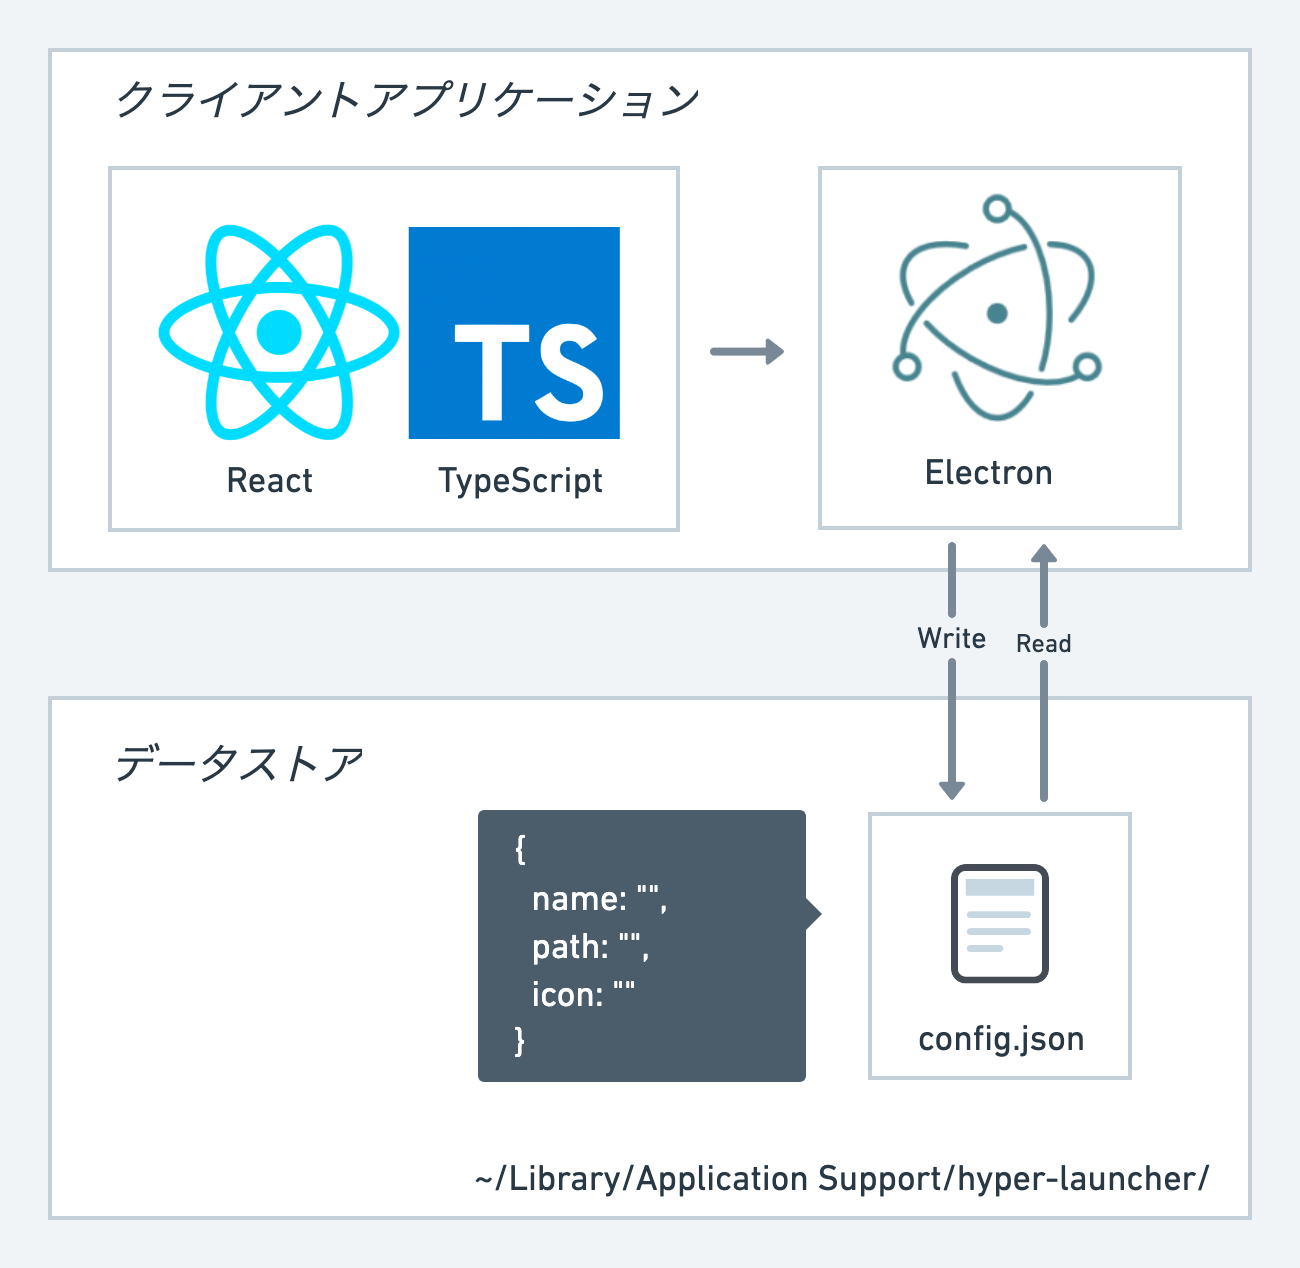
\includegraphics[width=100mm]{images/system}}
    \end{center}
    \caption{システムの構成}
    \label{fig:system}
\end{figure}

\section{クライアントアプリケーション}

クライアントアプリケーションはTypeScript及びReactなどのWeb技術によって実装されており、macOSのデスクトップアプリケーションとして動作する。

\subsection{Electron}

ElectronはHTML、JavaScript、CSSを用いてクロスプラットフォームなデスクトプアプリケーションを作成することができるソフトウェアフレームワークである。Electron自体はChromiumとNode.jsを使用しておりWeb技術のみで開発が完結するのが利点である。ElectronのAPIではグローバルなキーイベントのハンドリングを行えることに加え、アプリケーションの起動やアクティブ化なども操作できるため、ランチャーを作るにあたってとても有用なフレームワークである。

\subsection{AppleScript}

Web技術のみでは難しい部分についてはAppleScriptによって実装した。masOSにはosascriptと呼ばれるシェルスクリプトが存在し、これを利用することでNode.jsからAppleScriptを呼び出すことができる。AppleScriptを使用することで、起動中のアプリケーションや特定のアプリケーションがアクティブかどうかといった情報を取得することができるようになる。これによってデスクトップアプリケーションとして十分な機能を実装することができた。ただし実行するために毎回子プロセスを立ち上げるため、何も考えずに使用してしまうとラグが発生してしまうこととなる。

\section{データストア}

ユーザーが登録した情報は、Electronが定義するユーザーデータ領域(~/Library/Application Support/hyper-launcher/)にJSONファイルとして永続化されている。データのやり取りが全てローカルで完結するため、オフラインでも使用できようになっている。データはホットキーの数字をキーにし対応する値として配列を持ったオブジェクトになっており、それぞれアプリケーションの名前、パス、そしてbase64エンコードされたアイコンの3つを保持している。これにより単一のキーに対して複数のアプリケーションを登録することが可能となっている。以下にその例を示す。ただしiconのbase64文字列と中間部分は長くなるため省略した。

\begin{lstlisting}[caption=config.json]
{
  "shortcut": {
    "1": [
      {
        "name": "ForkLift",
        "path": "/Applications/ForkLift.app",
        "icon": "***************************"
      }
    ],
    "2": [
      {
        "name": "Hyper",
        "path": "/Applications/Hyper.app",
        "icon": "***************************"
      }
    ],
    
    ・・・
    
    "9": [
      {
        "name": "Hyper Launcher",
        "path": "/Applications/Hyper Launcher.app",
        "icon": "***************************"
      }
    ],
  }
}
\end{lstlisting}